% Options for packages loaded elsewhere
\PassOptionsToPackage{unicode}{hyperref}
\PassOptionsToPackage{hyphens}{url}
%
\documentclass[
]{article}
\usepackage{lmodern}
\usepackage{amssymb,amsmath}
\usepackage{ifxetex,ifluatex}
\ifnum 0\ifxetex 1\fi\ifluatex 1\fi=0 % if pdftex
  \usepackage[T1]{fontenc}
  \usepackage[utf8]{inputenc}
  \usepackage{textcomp} % provide euro and other symbols
\else % if luatex or xetex
  \usepackage{unicode-math}
  \defaultfontfeatures{Scale=MatchLowercase}
  \defaultfontfeatures[\rmfamily]{Ligatures=TeX,Scale=1}
\fi
% Use upquote if available, for straight quotes in verbatim environments
\IfFileExists{upquote.sty}{\usepackage{upquote}}{}
\IfFileExists{microtype.sty}{% use microtype if available
  \usepackage[]{microtype}
  \UseMicrotypeSet[protrusion]{basicmath} % disable protrusion for tt fonts
}{}
\makeatletter
\@ifundefined{KOMAClassName}{% if non-KOMA class
  \IfFileExists{parskip.sty}{%
    \usepackage{parskip}
  }{% else
    \setlength{\parindent}{0pt}
    \setlength{\parskip}{6pt plus 2pt minus 1pt}}
}{% if KOMA class
  \KOMAoptions{parskip=half}}
\makeatother
\usepackage{xcolor}
\IfFileExists{xurl.sty}{\usepackage{xurl}}{} % add URL line breaks if available
\IfFileExists{bookmark.sty}{\usepackage{bookmark}}{\usepackage{hyperref}}
\hypersetup{
  pdftitle={Overview of the Package trinROC},
  pdfauthor={Samuel Noll, Reinhard Furrer, Benjamin Reiser and Christos T. Nakas},
  hidelinks,
  pdfcreator={LaTeX via pandoc}}
\urlstyle{same} % disable monospaced font for URLs
\usepackage[margin=1in]{geometry}
\usepackage{color}
\usepackage{fancyvrb}
\newcommand{\VerbBar}{|}
\newcommand{\VERB}{\Verb[commandchars=\\\{\}]}
\DefineVerbatimEnvironment{Highlighting}{Verbatim}{commandchars=\\\{\}}
% Add ',fontsize=\small' for more characters per line
\usepackage{framed}
\definecolor{shadecolor}{RGB}{248,248,248}
\newenvironment{Shaded}{\begin{snugshade}}{\end{snugshade}}
\newcommand{\AlertTok}[1]{\textcolor[rgb]{0.94,0.16,0.16}{#1}}
\newcommand{\AnnotationTok}[1]{\textcolor[rgb]{0.56,0.35,0.01}{\textbf{\textit{#1}}}}
\newcommand{\AttributeTok}[1]{\textcolor[rgb]{0.77,0.63,0.00}{#1}}
\newcommand{\BaseNTok}[1]{\textcolor[rgb]{0.00,0.00,0.81}{#1}}
\newcommand{\BuiltInTok}[1]{#1}
\newcommand{\CharTok}[1]{\textcolor[rgb]{0.31,0.60,0.02}{#1}}
\newcommand{\CommentTok}[1]{\textcolor[rgb]{0.56,0.35,0.01}{\textit{#1}}}
\newcommand{\CommentVarTok}[1]{\textcolor[rgb]{0.56,0.35,0.01}{\textbf{\textit{#1}}}}
\newcommand{\ConstantTok}[1]{\textcolor[rgb]{0.00,0.00,0.00}{#1}}
\newcommand{\ControlFlowTok}[1]{\textcolor[rgb]{0.13,0.29,0.53}{\textbf{#1}}}
\newcommand{\DataTypeTok}[1]{\textcolor[rgb]{0.13,0.29,0.53}{#1}}
\newcommand{\DecValTok}[1]{\textcolor[rgb]{0.00,0.00,0.81}{#1}}
\newcommand{\DocumentationTok}[1]{\textcolor[rgb]{0.56,0.35,0.01}{\textbf{\textit{#1}}}}
\newcommand{\ErrorTok}[1]{\textcolor[rgb]{0.64,0.00,0.00}{\textbf{#1}}}
\newcommand{\ExtensionTok}[1]{#1}
\newcommand{\FloatTok}[1]{\textcolor[rgb]{0.00,0.00,0.81}{#1}}
\newcommand{\FunctionTok}[1]{\textcolor[rgb]{0.00,0.00,0.00}{#1}}
\newcommand{\ImportTok}[1]{#1}
\newcommand{\InformationTok}[1]{\textcolor[rgb]{0.56,0.35,0.01}{\textbf{\textit{#1}}}}
\newcommand{\KeywordTok}[1]{\textcolor[rgb]{0.13,0.29,0.53}{\textbf{#1}}}
\newcommand{\NormalTok}[1]{#1}
\newcommand{\OperatorTok}[1]{\textcolor[rgb]{0.81,0.36,0.00}{\textbf{#1}}}
\newcommand{\OtherTok}[1]{\textcolor[rgb]{0.56,0.35,0.01}{#1}}
\newcommand{\PreprocessorTok}[1]{\textcolor[rgb]{0.56,0.35,0.01}{\textit{#1}}}
\newcommand{\RegionMarkerTok}[1]{#1}
\newcommand{\SpecialCharTok}[1]{\textcolor[rgb]{0.00,0.00,0.00}{#1}}
\newcommand{\SpecialStringTok}[1]{\textcolor[rgb]{0.31,0.60,0.02}{#1}}
\newcommand{\StringTok}[1]{\textcolor[rgb]{0.31,0.60,0.02}{#1}}
\newcommand{\VariableTok}[1]{\textcolor[rgb]{0.00,0.00,0.00}{#1}}
\newcommand{\VerbatimStringTok}[1]{\textcolor[rgb]{0.31,0.60,0.02}{#1}}
\newcommand{\WarningTok}[1]{\textcolor[rgb]{0.56,0.35,0.01}{\textbf{\textit{#1}}}}
\usepackage{graphicx}
\makeatletter
\def\maxwidth{\ifdim\Gin@nat@width>\linewidth\linewidth\else\Gin@nat@width\fi}
\def\maxheight{\ifdim\Gin@nat@height>\textheight\textheight\else\Gin@nat@height\fi}
\makeatother
% Scale images if necessary, so that they will not overflow the page
% margins by default, and it is still possible to overwrite the defaults
% using explicit options in \includegraphics[width, height, ...]{}
\setkeys{Gin}{width=\maxwidth,height=\maxheight,keepaspectratio}
% Set default figure placement to htbp
\makeatletter
\def\fps@figure{htbp}
\makeatother
\setlength{\emergencystretch}{3em} % prevent overfull lines
\providecommand{\tightlist}{%
  \setlength{\itemsep}{0pt}\setlength{\parskip}{0pt}}
\setcounter{secnumdepth}{-\maxdimen} % remove section numbering
\ifluatex
  \usepackage{selnolig}  % disable illegal ligatures
\fi
\newlength{\cslhangindent}
\setlength{\cslhangindent}{1.5em}
\newlength{\csllabelwidth}
\setlength{\csllabelwidth}{3em}
\newenvironment{CSLReferences}[3] % #1 hanging-ident, #2 entry spacing
 {% don't indent paragraphs
  \setlength{\parindent}{0pt}
  % turn on hanging indent if param 1 is 1
  \ifodd #1 \everypar{\setlength{\hangindent}{\cslhangindent}}\ignorespaces\fi
  % set entry spacing
  \ifnum #2 > 0
  \setlength{\parskip}{#2\baselineskip}
  \fi
 }%
 {}
\usepackage{calc} % for \widthof, \maxof
\newcommand{\CSLBlock}[1]{#1\hfill\break}
\newcommand{\CSLLeftMargin}[1]{\parbox[t]{\maxof{\widthof{#1}}{\csllabelwidth}}{#1}}
\newcommand{\CSLRightInline}[1]{\parbox[t]{\linewidth}{#1}}
\newcommand{\CSLIndent}[1]{\hspace{\cslhangindent}#1}

\title{Overview of the Package \texttt{trinROC}}
\author{Samuel Noll, Reinhard Furrer, Benjamin Reiser and Christos T.
Nakas}
\date{2021-01-04}

\begin{document}
\maketitle

The package \texttt{trinROC} helps to assess three-class Receiver
Operating Characteristic (ROC) type data. It provides functions for
three statistical tests as described in Noll et al. (2019) along with
functions for Exploratory Data Analysis (EDA) and visualization.

We assume that the reader has some background in ROC analysis as well as
some understanding of the terminology associated with Area Under the ROC
Curve (AUC) and Volume Under the ROC Surface (VUS) indices. See Nakas
(2014) or Noll et al. (2019) for a concise overview.

This vignette consists of the following parts:

\begin{itemize}
\tightlist
\item
  Short background of the tests
\item
  Testing and comparing markers
\item
  Calculating empirical power curves
\item
  Additional functionality of the package
\end{itemize}

The package also contains two small data sets \texttt{cancer} and
\texttt{krebs} mimicking results of clinical studies. The datasets are
fairly small and used in this vignette (and in the examples of the help
files) to illustrate the functionality of the functions.

\hypertarget{short-background-of-the-tests}{%
\section{Short background of the
tests}\label{short-background-of-the-tests}}

We assume a three-class setting, where one or more classifier yields
measurements \(X = x\) on a continuous scale for the groups of healthy
(\(D^-\)), intermediate (\(D^0\)) and diseased (\(D^+\)) individuals. By
convention, larger values of \(x\) represent a more severe status of the
disease. The package \texttt{trinROC} provides statistical tests to
assess the discriminatory power of such classifiers. These tests are:

\begin{itemize}
\tightlist
\item
  Trinormal based ROC test (\texttt{trinROC.test}), developed by Noll et
  al. (2019);
\item
  Trinormal VUS test (\texttt{trinVUS.test}), developed by Xiong et al.
  (2007);
\item
  Bootstrap test, (\texttt{boot.test}), developed by Nakas and
  Yiannoutsos (2004).
\end{itemize}

In this document, we refer to the tests by the corresponding R function
name. All tests can assess a single classifier, as well as compare two
paired or unpaired classifiers.

As their names suggest, the underlying testing approach is different and
either based on VUS or on ROC. Hence, their null hypotheses differ as
well, as illustrated now.

\hypertarget{vus-based-statistical-tests}{%
\subsection{VUS based statistical
tests}\label{vus-based-statistical-tests}}

Given two classifiers, \texttt{boot.test} and \texttt{trinVUS.test} are
based on the null hypothesis \(VUS_1 = VUS_2\) with the \(Z\)-statistic

\begin{align*}
Z =  \frac{\widehat{VUS}_1 - \widehat{VUS}_2}{\sqrt{\widehat{Var}(\widehat{VUS}_1) + \widehat{Var}(\widehat{VUS}_2) - 2 \widehat{Cov}(\widehat{VUS}_1,\widehat{VUS}_2)}}.
\end{align*}

If the data of the two classifiers is unpaired, the term
\(Cov(VUS_1,VUS_2)\) is zero. If a single classifier is investigated,
the null hypothesis is \(VUS_1 = 1/6\) with the \(Z\)-statistic

\begin{align*}
Z =  \frac{\widehat{VUS}_1 - 1/6}{\sqrt{\widehat{Var}(\widehat{VUS}_1)}},
\end{align*}

which is equivalent to compared the VUS of the classifier to the volume
of an uninformative classifier. Details about the estimators are given
in the aforementioned papers.

\hypertarget{the-trinormal-based-roc-test}{%
\subsection{The trinormal based ROC
test}\label{the-trinormal-based-roc-test}}

In the trinormal model, the ROC surface is given by

\begin{align*}
ROC(t_-,t_+) = \Phi \left(\frac{\Phi^{-1} (1-t_+) + d}{ c} \right) - \Phi \left(\frac{\Phi^{-1} (t_-)+b}{a} \right),
\end{align*}

where \(\Phi\) is the cdf of the standard normal distribution and \(a\),
\(b\), \(c\) and \(d\) are functions of the means and standard
deviations of the three groups:

\begin{align*} 
a = \frac{{\sigma}_0}{{\sigma}_-}, \qquad b = \frac{ {\mu}_- - {\mu}_0}{{\sigma}_-}, \qquad 
c = \frac{{\sigma}_0}{{\sigma}_+}, \qquad d =  \frac{ {\mu}_+ - {\mu}_0}{{\sigma}_+}.
\end{align*}

Given two classifiers, \texttt{trinROC.test} investigates the shape of
the two ROC surfaces. Hence, the resulting null hypothesis is
\(a_1=a_2\), \(b_1=b_2\), \(c_1=c_2\) and \(d_1=d_2\), i.e., the the
surfaces have the same shape. Under the null hypothesis, the test
statistic

\begin{align*} 
 \chi^2 =  
 \begin{pmatrix} \widehat{a}_1 - \widehat{a}_2 &\widehat{b}_1 -\widehat{b}_2 & \widehat{c}_1-\widehat{c}_2 & \widehat{d}_1-\widehat{d}_2 \end{pmatrix}
 { \widehat{\boldsymbol{W}}}^{-1}
   \begin{pmatrix} \widehat{a}_1 - \widehat{a}_2 \\
    \widehat{b}_1 - \widehat{b}_2 \\ \widehat{c}_1-\widehat{c}_2 \\ \widehat{d}_1- \widehat{d}_2 \end{pmatrix},
\end{align*}

is distributed approximately as a chi-squared random variables with four
degrees of freedom, where \(\widehat{\boldsymbol{W}}\) contains the
corresponding estimated variances and covariances. The test rejects if
\(\chi^2 > \chi_{\alpha}^2\), i.e., if the test statistics exceeds the
chi-squared quantile with four degrees of freedom of a pre-defined
confidence level \(\alpha\).

When the data is unpaired, \(\widehat{a}_1\), \(\widehat{b}_1\),
\(\widehat{c}_1\), \(\widehat{d}_1\) are independent from
\(\widehat{a}_2\), \(\widehat{b}_2\), \(\widehat{c}_2\),
\(\widehat{d}_2\), respectively, and hence every combination of
covariances between them is zero.

It is also possible to investigate a single classifier with the above
method. Instead of an existing second classifier, we compare the
estimates \(\widehat{a}_1\) , \(\widehat{b}_1\), \(\widehat{c}_1\) and
\(\widehat{d}_1\) of a single marker with those from an artificial
marker. If we want to detect whether a single marker is significantly
better in allocating individuals to the three classes than a random
allocation function we would set the parameters of our null hypothesis
\(a_{Ho} = 1= c_{Ho}\), as we assume equal spread in the classes and
\(b_{Ho} = 0 = d_{Ho}\), as we impose equal means. This yields the null
hypothesis \(a_1=1\), \(b_1=0\), \(c_1=1\), \(d_1=0\), which leads to
the chi-squared test

\begin{align*} 
{\chi}^2 = & 
 \begin{pmatrix} \widehat{a}_1 -1 & \widehat{b}_1 & \widehat{c}_1 -1 & \widehat{d}_1 \end{pmatrix}
  \widehat{\boldsymbol{W}}^{-1}
   \begin{pmatrix} \widehat{a}_1 -1 \\ \widehat{b}_1 \\ \widehat{c}_1 - 1 \\ \widehat{d}_1 \end{pmatrix}.
\end{align*}

\hypertarget{testing-and-comparing-markers}{%
\section{Testing and comparing
markers}\label{testing-and-comparing-markers}}

We now illustrate the use of the test functions with the artificial
dataset \texttt{cancer}.

\begin{Shaded}
\begin{Highlighting}[]
\FunctionTok{data}\NormalTok{(cancer)}
\FunctionTok{str}\NormalTok{(cancer)}
\CommentTok{\#\textgreater{} \textquotesingle{}data.frame\textquotesingle{}:    100 obs. of  10 variables:}
\CommentTok{\#\textgreater{}  $ trueClass: Factor w/ 3 levels "healthy","intermediate",..: 3 3 3 3 3 3 3 3 3 3 ...}
\CommentTok{\#\textgreater{}  $ Class1   : num  1.42 1.69 1.08 1.79 1.46 0.1 1.91 2.57 1 1.87 ...}
\CommentTok{\#\textgreater{}  $ Class2   : num  2.31 2.36 1.72 2.34 1.97 0.74 2.82 2.71 1.67 2.51 ...}
\CommentTok{\#\textgreater{}  $ Class3   : num  {-}4647 {-}3694 {-}5119 {-}6352 {-}11509 ...}
\CommentTok{\#\textgreater{}  $ Class4   : num  {-}1622958 {-}1591840 {-}2299714 {-}2050907 {-}2629864 ...}
\CommentTok{\#\textgreater{}  $ Class5   : num  {-}476 {-}473 {-}618 {-}564 {-}901 ...}
\CommentTok{\#\textgreater{}  $ Class6   : num  12.36 8.81 9.15 5.52 11.85 ...}
\CommentTok{\#\textgreater{}  $ Class7   : num  2.48 4.38 2.3 2.41 4.68 1.34 3.18 2.35 1.83 2.83 ...}
\CommentTok{\#\textgreater{}  $ Class8   : num  3.02 2.98 2.94 3.01 2.93 2.95 3.02 3.03 2.93 3.06 ...}
\CommentTok{\#\textgreater{}  $ Class9   : num  {-}0.75 {-}0.86 {-}1.31 {-}0.27 {-}1.71 {-}1.39 {-}0.46 {-}1.06 {-}2.19 {-}0.91 ...}
\end{Highlighting}
\end{Shaded}

The first column is a factor indicating the (true) class membership of
each individual. The three levels have to be ordered according to
heaviness of disease, i.e., healthy, intermediate and diseased (nor the
names nor the sorting of the elements plays a role). The other columns
contain the measurements yielded by Classifier 1 to 9. Further we note
that some columns where multiplied by \(-1\) in order to fulfill the
convention that more diseased individuals have (in general) higher
measurements.

\hypertarget{single-marker-assessment}{%
\subsection{Single marker assessment}\label{single-marker-assessment}}

For illustration, let us assess \texttt{Class2} of the data set
\texttt{cancer} using the function \texttt{trinROC.test}.

\begin{Shaded}
\begin{Highlighting}[]
\NormalTok{out }\OtherTok{\textless{}{-}} \FunctionTok{trinROC.test}\NormalTok{(}\AttributeTok{dat =}\NormalTok{ cancer[,}\FunctionTok{c}\NormalTok{(}\StringTok{"trueClass"}\NormalTok{,}\StringTok{"Class2"}\NormalTok{)])}
\NormalTok{out}
\CommentTok{\#\textgreater{} }
\CommentTok{\#\textgreater{}  Trinormal based ROC test for single classifier assessment}
\CommentTok{\#\textgreater{} }
\CommentTok{\#\textgreater{} data:  healthy  intermediate  diseased  of  Class2}
\CommentTok{\#\textgreater{} Chi{-}Squared test = 47.1, df = 4, p{-}value = 1.4e{-}09}
\CommentTok{\#\textgreater{} alternative hypothesis: true a1{-}a2, b1{-}b1, c1{-}c2 and d1{-}d2 is not equal to 0}
\CommentTok{\#\textgreater{} sample estimates:}
\CommentTok{\#\textgreater{}            VUS      a       b       c       d}
\CommentTok{\#\textgreater{} Class2 0.41582 1.8371 {-}1.2333 0.84364 0.56005}
\end{Highlighting}
\end{Shaded}

The function returns a list of class \texttt{"htest"}, similar to other
tests from the \texttt{stats} package. Additionally to the standard list
elements, we also obtain detailed information about data and the sample
estimates (VUS, and if applicable, estimates of \(a\), \(b\), \(c\) and
\(d\))

\begin{Shaded}
\begin{Highlighting}[]
\NormalTok{out[ }\FunctionTok{c}\NormalTok{(}\StringTok{"estimate"}\NormalTok{, }\StringTok{"Summary"}\NormalTok{, }\StringTok{"CovMat"}\NormalTok{)]}
\CommentTok{\#\textgreater{} $estimate}
\CommentTok{\#\textgreater{}            VUS      a       b       c       d}
\CommentTok{\#\textgreater{} Class2 0.41582 1.8371 {-}1.2333 0.84364 0.56005}
\CommentTok{\#\textgreater{} }
\CommentTok{\#\textgreater{} $Summary}
\CommentTok{\#\textgreater{}               n     mu      sd}
\CommentTok{\#\textgreater{} healthy      38 1.3603 0.23525}
\CommentTok{\#\textgreater{} intermediate 25 1.6504 0.43217}
\CommentTok{\#\textgreater{} diseased     37 1.9373 0.51227}
\CommentTok{\#\textgreater{} }
\CommentTok{\#\textgreater{} $CovMat}
\CommentTok{\#\textgreater{}           [,1]      [,2]      [,3]      [,4]}
\CommentTok{\#\textgreater{} [1,]  0.111904 {-}0.029812 0.0309968 0.0000000}
\CommentTok{\#\textgreater{} [2,] {-}0.029812  0.181325 0.0000000 0.0619936}
\CommentTok{\#\textgreater{} [3,]  0.030997  0.000000 0.0238526 0.0063849}
\CommentTok{\#\textgreater{} [4,]  0.000000  0.061994 0.0063849 0.0597349}
\end{Highlighting}
\end{Shaded}

More specifically:

\begin{itemize}
\tightlist
\item
  \texttt{\$Summary} displays a summary table of \(n_\ell\),
  \(\mu_\ell\) and \(\sigma_\ell\) for \(\ell = -,0,+\), the three
  classes \(D^-\), \(D^0\) and \(D^+\).
\item
  \texttt{\$CovMat} or \texttt{\$Sigma} displays the covariance matrix
  of the test.
\end{itemize}

The tests \texttt{trinVUS.test} and \texttt{boot.test} work analogously.

\begin{Shaded}
\begin{Highlighting}[]
\NormalTok{ROCsin }\OtherTok{\textless{}{-}} \FunctionTok{trinROC.test}\NormalTok{(}\AttributeTok{dat =}\NormalTok{ cancer[,}\FunctionTok{c}\NormalTok{(}\DecValTok{1}\NormalTok{,}\DecValTok{3}\NormalTok{)])}
\NormalTok{VUSsin }\OtherTok{\textless{}{-}} \FunctionTok{trinVUS.test}\NormalTok{(}\AttributeTok{dat =}\NormalTok{ cancer[,}\FunctionTok{c}\NormalTok{(}\DecValTok{1}\NormalTok{,}\DecValTok{3}\NormalTok{)])}
\NormalTok{bootsin }\OtherTok{\textless{}{-}} \FunctionTok{boot.test}\NormalTok{(}\AttributeTok{dat =}\NormalTok{ cancer[,}\FunctionTok{c}\NormalTok{(}\DecValTok{1}\NormalTok{,}\DecValTok{3}\NormalTok{)], }\AttributeTok{n.boot =} \DecValTok{250}\NormalTok{)}

\FunctionTok{c}\NormalTok{( ROCsin}\SpecialCharTok{$}\NormalTok{p.value, VUSsin}\SpecialCharTok{$}\NormalTok{p.value, bootsin}\SpecialCharTok{$}\NormalTok{p.value)}
\CommentTok{\#\textgreater{} [1] 1.4499e{-}09 7.7041e{-}06 2.0081e{-}05}
\end{Highlighting}
\end{Shaded}

The test functions \texttt{trinROC.test}, \texttt{trinVUS.test} and
\texttt{boot.test} handle either data frames that have the same form as
\texttt{cancer} or single vectors specifying the three groups. For
example

\begin{Shaded}
\begin{Highlighting}[]
\NormalTok{(x1 }\OtherTok{\textless{}{-}} \FunctionTok{with}\NormalTok{(cancer, cancer[trueClass}\SpecialCharTok{==}\StringTok{"healthy"}\NormalTok{, }\DecValTok{3}\NormalTok{]))}
\CommentTok{\#\textgreater{}  [1] 1.21 1.50 1.10 0.96 0.93 1.52 1.74 1.55 0.88 1.43 1.43 1.36 1.38 1.36 1.43 1.38 1.32 1.29 0.96 1.23 1.19}
\CommentTok{\#\textgreater{} [22] 1.40 1.75 1.44 1.32 1.73 1.62 1.39 1.22 1.28 1.56 1.05 1.42 1.58 1.69 1.47 1.55 1.07}
\NormalTok{(y1 }\OtherTok{\textless{}{-}} \FunctionTok{with}\NormalTok{(cancer, cancer[trueClass}\SpecialCharTok{==}\StringTok{"intermediate"}\NormalTok{, }\DecValTok{3}\NormalTok{]))}
\CommentTok{\#\textgreater{}  [1] 1.58 1.98 1.63 1.32 1.85 2.07 2.03 0.93 1.53 1.91 2.09 2.40 1.79 1.37 1.16 1.81 2.47 1.60 1.91 0.93 1.47}
\CommentTok{\#\textgreater{} [22] 1.56 0.99 1.41 1.47}
\NormalTok{(z1 }\OtherTok{\textless{}{-}} \FunctionTok{with}\NormalTok{(cancer, cancer[trueClass}\SpecialCharTok{==}\StringTok{"diseased"}\NormalTok{, }\DecValTok{3}\NormalTok{]))}
\CommentTok{\#\textgreater{}  [1] 2.31 2.36 1.72 2.34 1.97 0.74 2.82 2.71 1.67 2.51 2.18 2.47 1.88 1.89 1.69 1.35 1.90 2.33 1.79 2.03 2.24}
\CommentTok{\#\textgreater{} [22] 2.01 1.01 2.88 1.68 1.13 1.11 1.23 1.92 1.69 2.18 2.37 1.82 1.59 1.94 2.20 2.02}
\NormalTok{ROCsin2 }\OtherTok{\textless{}{-}} \FunctionTok{trinROC.test}\NormalTok{(x1, y1, z1)}
\DocumentationTok{\#\# All numbers are equal; sole difference is name of data:}
\FunctionTok{all.equal}\NormalTok{(ROCsin, ROCsin2, }\AttributeTok{check.attributes =} \ConstantTok{FALSE}\NormalTok{)}
\CommentTok{\#\textgreater{} [1] "Component \textbackslash{}"data.name\textbackslash{}": 1 string mismatch"}
\end{Highlighting}
\end{Shaded}

\hypertarget{comparison-of-two-paired-or-unpaired-markers}{%
\subsection{Comparison of two paired or unpaired
markers}\label{comparison-of-two-paired-or-unpaired-markers}}

Assume we now want to compare \texttt{Class2} with \texttt{Class4}. If
the data is paired, we take this into account by setting
\texttt{paired\ =\ TRUE}.

\begin{Shaded}
\begin{Highlighting}[]
\NormalTok{ROCcomp }\OtherTok{\textless{}{-}} \FunctionTok{trinROC.test}\NormalTok{(}\AttributeTok{dat =}\NormalTok{ cancer[,}\FunctionTok{c}\NormalTok{(}\DecValTok{1}\NormalTok{,}\DecValTok{3}\NormalTok{,}\DecValTok{5}\NormalTok{)], }\AttributeTok{paired =} \ConstantTok{TRUE}\NormalTok{)}
\NormalTok{ROCcom  }\OtherTok{\textless{}{-}} \FunctionTok{trinROC.test}\NormalTok{(}\AttributeTok{dat =}\NormalTok{ cancer[,}\FunctionTok{c}\NormalTok{(}\DecValTok{1}\NormalTok{,}\DecValTok{3}\NormalTok{,}\DecValTok{5}\NormalTok{)])}

\NormalTok{ROCcomp}\SpecialCharTok{$}\NormalTok{p.value}
\CommentTok{\#\textgreater{} [1] 0.03448}
\NormalTok{ROCcom}\SpecialCharTok{$}\NormalTok{p.value}
\CommentTok{\#\textgreater{} [1] 0.13736}
\CommentTok{\# is equal to:}
\NormalTok{x2 }\OtherTok{\textless{}{-}} \FunctionTok{with}\NormalTok{(cancer, cancer[trueClass}\SpecialCharTok{==}\StringTok{"healthy"}\NormalTok{, }\DecValTok{5}\NormalTok{])}
\NormalTok{y2 }\OtherTok{\textless{}{-}} \FunctionTok{with}\NormalTok{(cancer, cancer[trueClass}\SpecialCharTok{==}\StringTok{"intermediate"}\NormalTok{, }\DecValTok{5}\NormalTok{])}
\NormalTok{z2 }\OtherTok{\textless{}{-}} \FunctionTok{with}\NormalTok{(cancer, cancer[trueClass}\SpecialCharTok{==}\StringTok{"diseased"}\NormalTok{, }\DecValTok{5}\NormalTok{])}
\NormalTok{ROCcomp2 }\OtherTok{\textless{}{-}} \FunctionTok{trinROC.test}\NormalTok{(x1, y1, z1, x2, y2, z2, }\AttributeTok{paired =} \ConstantTok{TRUE}\NormalTok{)}
\end{Highlighting}
\end{Shaded}

Beside the argument \texttt{paired} it is also possible to adjust the
confidence level (default is \texttt{conf.level\ =\ 0.95}). For the
\texttt{trinVUS.test} and the \texttt{boot.test} one can also specify
the alternative hypothesis
(\texttt{alternative\ =\ c("two.sided",\ "less",\ "greater")}). This not
possible for the \texttt{trinROC.test}, as this is a chi-squared test.

\hypertarget{calcuating-empirical-power-curves}{%
\section{Calcuating empirical power
curves}\label{calcuating-empirical-power-curves}}

In this section, we outline the code used to construct the empirical
power curves of Figures 2, 3 etc. For simplicity, here and in the paper,
we set the mean and variances if the healthy group to zero and one,
respectively. The variances of the intermediate and diseased groups are
pre-specified (``slight crossing''). Finally the remaining means are
found based on a desired VUS.

\begin{Shaded}
\begin{Highlighting}[]
\FunctionTok{require}\NormalTok{( ggplot2, }\AttributeTok{quietly =} \ConstantTok{TRUE}\NormalTok{)}
\FunctionTok{require}\NormalTok{( MASS, }\AttributeTok{quietly =} \ConstantTok{TRUE}\NormalTok{)}
\NormalTok{N }\OtherTok{\textless{}{-}} \DecValTok{25}
\NormalTok{reps }\OtherTok{\textless{}{-}} \DecValTok{99}                    \CommentTok{\# Is set to 1000 in the paper}
\NormalTok{rho }\OtherTok{\textless{}{-}} \FloatTok{0.5}                    \CommentTok{\# paired setting if rho!=0}

\NormalTok{sd.y1 }\OtherTok{\textless{}{-}} \FloatTok{1.25}\NormalTok{;  sd.y2 }\OtherTok{\textless{}{-}} \FloatTok{1.5}  \CommentTok{\# this corresponds to medium crossing}
\NormalTok{sd.z1 }\OtherTok{\textless{}{-}} \FloatTok{1.5}\NormalTok{;   sd.z2 }\OtherTok{\textless{}{-}} \DecValTok{2}

\NormalTok{Vus }\OtherTok{\textless{}{-}} \FunctionTok{c}\NormalTok{(}\FloatTok{0.2}\NormalTok{, }\FloatTok{0.25}\NormalTok{, }\FloatTok{0.3}\NormalTok{, }\FloatTok{0.35}\NormalTok{, }\FloatTok{0.4}\NormalTok{, }\FloatTok{0.45}\NormalTok{)}
\NormalTok{lVus }\OtherTok{\textless{}{-}} \FunctionTok{length}\NormalTok{(Vus)}

\NormalTok{result }\OtherTok{\textless{}{-}} \FunctionTok{matrix}\NormalTok{(}\DecValTok{0}\NormalTok{, lVus, reps)}
\NormalTok{tmp }\OtherTok{\textless{}{-}} \FunctionTok{findmu}\NormalTok{(}\AttributeTok{sdy=}\NormalTok{sd.y1, }\AttributeTok{sdz=}\NormalTok{sd.z1, }\AttributeTok{VUS=}\NormalTok{Vus[}\DecValTok{1}\NormalTok{])}
\NormalTok{mom1 }\OtherTok{\textless{}{-}}\NormalTok{ tmp[,}\DecValTok{2}\NormalTok{]}
\FunctionTok{names}\NormalTok{(mom1) }\OtherTok{\textless{}{-}}\NormalTok{ tmp[,}\DecValTok{1}\NormalTok{]}
\ControlFlowTok{for}\NormalTok{ (m }\ControlFlowTok{in} \DecValTok{1}\SpecialCharTok{:}\NormalTok{lVus)\{            }\CommentTok{\# cycle over different VUS}
\NormalTok{  mom2 }\OtherTok{\textless{}{-}} \FunctionTok{findmu}\NormalTok{(}\AttributeTok{sdy=}\NormalTok{sd.y2, }\AttributeTok{sdz=}\NormalTok{sd.z2, }\AttributeTok{VUS=}\NormalTok{Vus[m])[,}\DecValTok{2}\NormalTok{]}
  \FunctionTok{names}\NormalTok{(mom2) }\OtherTok{\textless{}{-}}\NormalTok{ tmp[,}\DecValTok{1}\NormalTok{]}
  \ControlFlowTok{for}\NormalTok{( i }\ControlFlowTok{in} \DecValTok{1}\SpecialCharTok{:}\NormalTok{reps) \{         }\CommentTok{\# cycle over replicates}
\NormalTok{    SigmaX }\OtherTok{\textless{}{-}} \FunctionTok{matrix}\NormalTok{(}\FunctionTok{c}\NormalTok{(}\DecValTok{1}\NormalTok{, rho, rho, }\DecValTok{1}\NormalTok{), }\DecValTok{2}\NormalTok{, }\DecValTok{2}\NormalTok{)}
\NormalTok{    SigmaY }\OtherTok{\textless{}{-}} \FunctionTok{matrix}\NormalTok{(}\FunctionTok{c}\NormalTok{(sd.y1}\SpecialCharTok{\^{}}\DecValTok{2}\NormalTok{, sd.y1}\SpecialCharTok{*}\NormalTok{sd.y2}\SpecialCharTok{*}\NormalTok{rho,}
\NormalTok{                       sd.y1}\SpecialCharTok{*}\NormalTok{sd.y2}\SpecialCharTok{*}\NormalTok{rho, sd.y2}\SpecialCharTok{\^{}}\DecValTok{2}\NormalTok{), }\DecValTok{2}\NormalTok{, }\DecValTok{2}\NormalTok{)}
\NormalTok{    SigmaZ }\OtherTok{\textless{}{-}} \FunctionTok{matrix}\NormalTok{(}\FunctionTok{c}\NormalTok{(sd.z1}\SpecialCharTok{\^{}}\DecValTok{2}\NormalTok{, sd.z1}\SpecialCharTok{*}\NormalTok{sd.z2}\SpecialCharTok{*}\NormalTok{rho,}
\NormalTok{                       sd.z1}\SpecialCharTok{*}\NormalTok{sd.z2}\SpecialCharTok{*}\NormalTok{rho, sd.z2}\SpecialCharTok{\^{}}\DecValTok{2}\NormalTok{), }\DecValTok{2}\NormalTok{, }\DecValTok{2}\NormalTok{)}
\NormalTok{    x }\OtherTok{\textless{}{-}} \FunctionTok{mvrnorm}\NormalTok{(N, }\FunctionTok{c}\NormalTok{(}\DecValTok{0}\NormalTok{, }\DecValTok{0}\NormalTok{), SigmaX)}
\NormalTok{    y }\OtherTok{\textless{}{-}} \FunctionTok{mvrnorm}\NormalTok{(N, }\FunctionTok{c}\NormalTok{(mom1[}\StringTok{"muy"}\NormalTok{], mom2[}\StringTok{"muy"}\NormalTok{]), SigmaY)}
\NormalTok{    z }\OtherTok{\textless{}{-}} \FunctionTok{mvrnorm}\NormalTok{(N, }\FunctionTok{c}\NormalTok{(mom1[}\StringTok{"muz"}\NormalTok{], mom2[}\StringTok{"muz"}\NormalTok{]), SigmaZ)}

\NormalTok{    MT }\OtherTok{\textless{}{-}} \FunctionTok{trinROC.test}\NormalTok{(}\AttributeTok{x1 =}\NormalTok{ x[,}\DecValTok{1}\NormalTok{], }\AttributeTok{y1 =}\NormalTok{ y[,}\DecValTok{1}\NormalTok{], }\AttributeTok{z1 =}\NormalTok{ z[,}\DecValTok{1}\NormalTok{],}
                       \AttributeTok{x2 =}\NormalTok{ x[,}\DecValTok{2}\NormalTok{], }\AttributeTok{y2 =}\NormalTok{ y[,}\DecValTok{2}\NormalTok{], }\AttributeTok{z2 =}\NormalTok{ z[,}\DecValTok{2}\NormalTok{], }\AttributeTok{paired =}\NormalTok{ (rho}\SpecialCharTok{!=}\DecValTok{0}\NormalTok{))}
\NormalTok{    result[m,i] }\OtherTok{\textless{}{-}}\NormalTok{ MT}\SpecialCharTok{$}\NormalTok{p.value}
\NormalTok{  \}}
\NormalTok{\}}

\NormalTok{empPow }\OtherTok{\textless{}{-}} \FunctionTok{data.frame}\NormalTok{(}\AttributeTok{x =}\NormalTok{ Vus, }\AttributeTok{value =} \FunctionTok{rowMeans}\NormalTok{(result}\SpecialCharTok{\textless{}}\FloatTok{0.05}\NormalTok{))}
\FunctionTok{ggplot}\NormalTok{(}\AttributeTok{data =}\NormalTok{ empPow, }\FunctionTok{aes}\NormalTok{(}\AttributeTok{x =}\NormalTok{ Vus, }\AttributeTok{y =}\NormalTok{ value)) }\SpecialCharTok{+} \FunctionTok{geom\_line}\NormalTok{() }\SpecialCharTok{+} \FunctionTok{geom\_point}\NormalTok{() }\SpecialCharTok{+}
    \FunctionTok{ylab}\NormalTok{(}\StringTok{"Empirical Power"}\NormalTok{) }\SpecialCharTok{+} \FunctionTok{scale\_y\_continuous}\NormalTok{(}\AttributeTok{breaks =} \FunctionTok{c}\NormalTok{(}\FloatTok{0.05}\NormalTok{, }\FloatTok{0.25}\NormalTok{, }\FloatTok{0.5}\NormalTok{, }\DecValTok{1}\NormalTok{))}
\end{Highlighting}
\end{Shaded}

\includegraphics{trinROC_vignette_files/figure-latex/emppow-1.pdf}

For the simulation study, we additionally calculated the p-values of
\texttt{boot.test} and varied \(VUS_1\), \(VUS_2\) and \(N\).

\hypertarget{additional-functionality-of-the-package}{%
\section{Additional functionality of the
package}\label{additional-functionality-of-the-package}}

In this section we discuss functions of the package \texttt{trinROC}
that help in the process of exploring, preparing and visualizing the
data in the context of ROC analysis.

\hypertarget{how-to-apply-the-eda-function}{%
\subsection{How to apply the EDA
function}\label{how-to-apply-the-eda-function}}

Formal statistical testing is typically preceded by an exploratory data
analysis. The function \texttt{roc.eda} serves this purpose and provides
three different viewpoints on its input data:

\begin{itemize}
\tightlist
\item
  It computes the empirical or trinormal VUS as well as the test
  statistic for a single marker investigation
\item
  It plots density, boxplots or scatter plots of the data according to
  the three classes
\item
  It plots the empirical or trinormal ROC surface, using the package
  \texttt{rgl}.
\end{itemize}

The last option can be turned off by setting \texttt{plotVUS\ =\ FALSE}.
If only the interactive three-dimensional plot is desired, one can also
use the functions \texttt{rocsurf.emp} for empirical ROC surfaces and
\texttt{rocsurf.trin} for trinormal ROC surfaces.

\begin{Shaded}
\begin{Highlighting}[]
\FunctionTok{data}\NormalTok{( cancer)}
\FunctionTok{roc.eda}\NormalTok{(}\AttributeTok{dat =}\NormalTok{ cancer[,}\FunctionTok{c}\NormalTok{(}\DecValTok{1}\NormalTok{,}\DecValTok{5}\NormalTok{)], }\AttributeTok{type =} \StringTok{"trinormal"}\NormalTok{, }\AttributeTok{plotVUS =} \ConstantTok{FALSE}\NormalTok{, }\AttributeTok{saveVUS =} \ConstantTok{TRUE}\NormalTok{)}
\end{Highlighting}
\end{Shaded}

\includegraphics{trinROC_vignette_files/figure-latex/roc.eda1-1.pdf}

\begin{verbatim}
#> 
#>  Data overview of trinormal ROC Classifier 
#> --------------------------------------------------------------------- 
#> 
#>  Applied tests: Trinormal based ROC and VUS test 
#>  Significance level: 0.05
#>  Alternative hypothesis: two.sided
#> --------------------------------------------------------------------- 
#>  data: healthy, intermediate and diseased
#> 
#> ROC test statistic: 25.421, ROC p.value: 4e-05
#>  VUS test statistic:  3.418 ,  VUS p.value:  0.00063 
#> 
#>  trinormal VUS:  0.344 
#> 
#> Parameters: 
#>      a   b   c   d   
#>      1.3766  -1.1808 1.101   0.1951  
#> ---------------------------------------------------------------------
\end{verbatim}

\begin{Shaded}
\begin{Highlighting}[]
\FunctionTok{roc.eda}\NormalTok{(}\AttributeTok{dat =}\NormalTok{ cancer[,}\FunctionTok{c}\NormalTok{(}\DecValTok{1}\NormalTok{,}\DecValTok{5}\NormalTok{)], }\AttributeTok{type =} \StringTok{"empirical"}\NormalTok{, }\AttributeTok{sep.dens =} \ConstantTok{TRUE}\NormalTok{, }\AttributeTok{scatter =} \ConstantTok{TRUE}\NormalTok{, }
        \AttributeTok{verbose =} \ConstantTok{FALSE}\NormalTok{)}
\end{Highlighting}
\end{Shaded}

\includegraphics{trinROC_vignette_files/figure-latex/roc.eda2-1.pdf}

\begin{Shaded}
\begin{Highlighting}[]
\DocumentationTok{\#\# is last call is equal to:}
\CommentTok{\# x \textless{}{-} with(cancer, cancer[trueClass=="healthy", 5])}
\CommentTok{\# y \textless{}{-} with(cancer, cancer[trueClass=="intermediate", 5])}
\CommentTok{\# z \textless{}{-} with(cancer, cancer[trueClass=="diseased", 5])}
\CommentTok{\# roc.eda(x, y, z, type = "trinormal")}
\end{Highlighting}
\end{Shaded}

By setting \texttt{plotVUS\ =\ TRUE} an interactive rgl plot window is
opened, displaying the ROC surface computed from the measurements.
Depending the argument \texttt{type} the empirical or trinormal ROC
surface is computed. The below Figures displays the empirical and
trinormal snapshot of the ROC surfaces of the example data used in this
section.

\begin{figure}
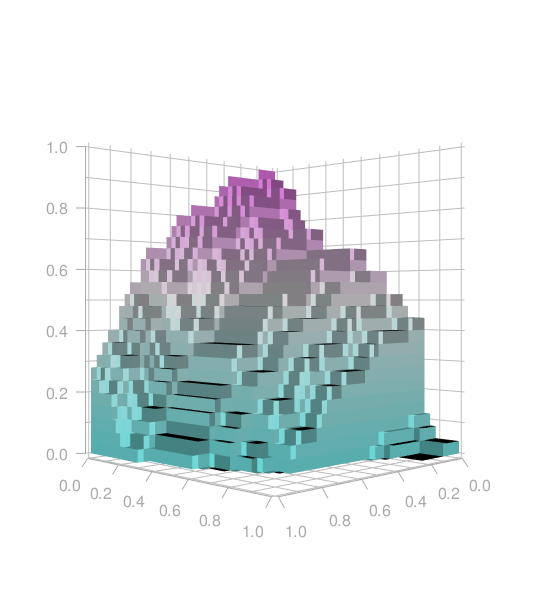
\includegraphics[width=0.45\linewidth]{Figures//empVUS} 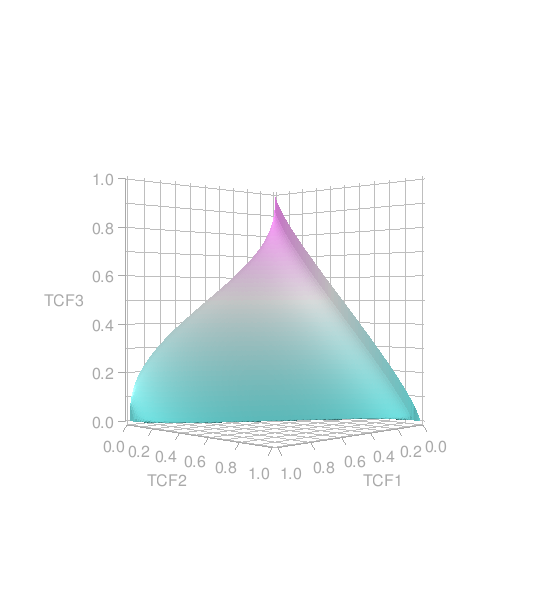
\includegraphics[width=0.45\linewidth]{Figures//trinVUS} \caption{Empirical and trinormal ROC surfaces}\label{fig:figsfigs}
\end{figure}

\hypertarget{computing-the-empirical-vus}{%
\subsection{Computing the (empirical)
VUS}\label{computing-the-empirical-vus}}

To calculate the VUS (empirical or estimate based on the trinormal
assumption) the following code can be used.

\begin{Shaded}
\begin{Highlighting}[]
\FunctionTok{data}\NormalTok{( cancer)}
\NormalTok{x }\OtherTok{\textless{}{-}} \FunctionTok{with}\NormalTok{(cancer, cancer[trueClass}\SpecialCharTok{==}\StringTok{"healthy"}\NormalTok{, }\DecValTok{5}\NormalTok{])}
\NormalTok{y }\OtherTok{\textless{}{-}} \FunctionTok{with}\NormalTok{(cancer, cancer[trueClass}\SpecialCharTok{==}\StringTok{"intermediate"}\NormalTok{, }\DecValTok{5}\NormalTok{])}
\NormalTok{z }\OtherTok{\textless{}{-}} \FunctionTok{with}\NormalTok{(cancer, cancer[trueClass}\SpecialCharTok{==}\StringTok{"diseased"}\NormalTok{, }\DecValTok{5}\NormalTok{])}
\FunctionTok{emp.vus}\NormalTok{(x, y, z)}
\CommentTok{\#\textgreater{} [1] 0.37741}
\FunctionTok{trinVUS.test}\NormalTok{(x, y, z)}\SpecialCharTok{$}\NormalTok{estimate}
\CommentTok{\#\textgreater{} VUS of Classifier 1 }
\CommentTok{\#\textgreater{}             0.34361}
\FunctionTok{trinROC.test}\NormalTok{(x, y, z)}\SpecialCharTok{$}\NormalTok{estimate[}\DecValTok{1}\NormalTok{]}
\CommentTok{\#\textgreater{}                  VUS}
\CommentTok{\#\textgreater{} Classifier1: 0.34361}
\end{Highlighting}
\end{Shaded}

The ROC surface itself is visualized using
\texttt{rocsurf.emp(x,\ y,\ z)} or \texttt{rocsurf.trin(x,\ y,\ z)}.

\hypertarget{transforming-non-normal-data-using-boxcoxroc}{%
\subsection{\texorpdfstring{Transforming non-normal data using
\texttt{boxcoxROC}}{Transforming non-normal data using boxcoxROC}}\label{transforming-non-normal-data-using-boxcoxroc}}

The trinormal model based test, \texttt{trinROC.test} or
\texttt{trinVUS.test} are build upon a normality assumption of the data.
If this assumption is violated, the trinormal tests may yield incorrect
results. A common way to test for normality is the
\texttt{shapiro.test}. If the hypothesis of normally distributed data is
rejected, there is a possibility to apply the function
\texttt{boxcoxROC} to the data. This function takes three vectors
\texttt{x}, \texttt{y} and \texttt{z} and computes a Box-Cox
transformation, see Box and Cox (1964) and Bantis et al. (2017).
Consider this short example:

\begin{Shaded}
\begin{Highlighting}[]
\FunctionTok{set.seed}\NormalTok{(}\DecValTok{712}\NormalTok{)}
\NormalTok{x }\OtherTok{\textless{}{-}} \FunctionTok{rchisq}\NormalTok{(}\DecValTok{20}\NormalTok{, }\DecValTok{2}\NormalTok{)}
\NormalTok{y }\OtherTok{\textless{}{-}} \FunctionTok{rchisq}\NormalTok{(}\DecValTok{20}\NormalTok{, }\DecValTok{6}\NormalTok{)}
\NormalTok{z }\OtherTok{\textless{}{-}} \FunctionTok{rchisq}\NormalTok{(}\DecValTok{20}\NormalTok{, }\DecValTok{10}\NormalTok{)}
\FunctionTok{boxcoxROC}\NormalTok{(x, y, z)}
\CommentTok{\#\textgreater{} {-}{-}{-}{-}{-}{-}{-}{-}{-}{-}{-}{-}{-}{-}{-}{-}{-}{-}{-}{-}{-}{-}{-}{-}{-}{-}{-}{-}{-}{-}{-}{-}{-}{-}{-}{-}{-}{-}{-}{-}{-}{-}{-}{-}{-}{-}{-}{-}{-}{-}{-}{-}{-}{-}{-}{-}{-}{-}{-}{-}{-}{-}{-}{-}{-}{-}{-}{-}{-} }
\CommentTok{\#\textgreater{}  Optimal lambda       = 0.15}
\CommentTok{\#\textgreater{}  Shift param. lambda2 = 0}
\CommentTok{\#\textgreater{} }
\CommentTok{\#\textgreater{}  Shapiro p{-}values for original data: }
\CommentTok{\#\textgreater{}  x = 0.00079639, y = 0.0058895, z = 0.56616}
\CommentTok{\#\textgreater{} }
\CommentTok{\#\textgreater{}  Shapiro p{-}values for Box{-}Cox transformed data: }
\CommentTok{\#\textgreater{}  x = 0.49498, y = 0.10501, z = 0.27073}
\CommentTok{\#\textgreater{} {-}{-}{-}{-}{-}{-}{-}{-}{-}{-}{-}{-}{-}{-}{-}{-}{-}{-}{-}{-}{-}{-}{-}{-}{-}{-}{-}{-}{-}{-}{-}{-}{-}{-}{-}{-}{-}{-}{-}{-}{-}{-}{-}{-}{-}{-}{-}{-}{-}{-}{-}{-}{-}{-}{-}{-}{-}{-}{-}{-}{-}{-}{-}{-}{-}{-}{-}{-}{-}}
\end{Highlighting}
\end{Shaded}

\hypertarget{an-omnibus-analysis-using-the-function-roc3.test}{%
\subsection{\texorpdfstring{An omnibus analysis using the function
\texttt{roc3.test}}{An omnibus analysis using the function roc3.test}}\label{an-omnibus-analysis-using-the-function-roc3.test}}

The function \texttt{roc3.test} computes every one by one combination of
classifiers it contains to a desired combination of the three
statistical tests \texttt{trinROC.test}, \texttt{trinVUS.test} and
\texttt{boot.test} in one step. Furthermore, single classifier
assessment tests are automatically computed as well. The output consists
of:

\begin{itemize}
\item
  Two data frames that contain information about each marker on its own.
  In the first data frame \texttt{overview} the markers are sorted by
  their empirical VUS, while in the second data frame they are shown in
  their original order.
\item
  For each statistical test that has been chosen, two strictly upper
  triangular matrices are returned, one containing the p-values and one
  the test values.
\end{itemize}

\begin{Shaded}
\begin{Highlighting}[]
\NormalTok{out }\OtherTok{\textless{}{-}} \FunctionTok{roc3.test}\NormalTok{(cancer[,}\DecValTok{1}\SpecialCharTok{:}\DecValTok{8}\NormalTok{], }\AttributeTok{type =} \FunctionTok{c}\NormalTok{(}\StringTok{"ROC"}\NormalTok{, }\StringTok{"VUS"}\NormalTok{), }\AttributeTok{paired =} \ConstantTok{TRUE}\NormalTok{)}
\NormalTok{out[}\FunctionTok{c}\NormalTok{(}\DecValTok{1}\NormalTok{,}\DecValTok{3}\NormalTok{)]}
\CommentTok{\#\textgreater{} $Overview}
\CommentTok{\#\textgreater{}                  Class6 Class1 Class2 Class3 Class4 Class5 Class7}
\CommentTok{\#\textgreater{} Charts           1.0000 2.0000 3.0000 4.0000 5.0000 6.0000 7.0000}
\CommentTok{\#\textgreater{} Emp. VUS         0.5317 0.4763 0.4411 0.4354 0.3774 0.3661 0.2918}
\CommentTok{\#\textgreater{} Trin. VUS        0.5557 0.4283 0.4158 0.4091 0.3436 0.3736 0.3440}
\CommentTok{\#\textgreater{} p.value ROC test 0.0000 0.0000 0.0000 0.0000 0.0000 0.0000 0.0000}
\CommentTok{\#\textgreater{} p.value VUS test 0.0000 0.0000 0.0000 0.0000 0.0006 0.0001 0.0007}
\CommentTok{\#\textgreater{} Nr. of NA\textquotesingle{}s      0.0000 0.0000 0.0000 0.0000 0.0000 0.0000 0.0000}
\CommentTok{\#\textgreater{} }
\CommentTok{\#\textgreater{} $P.values}
\CommentTok{\#\textgreater{} $P.values$trinROC}
\CommentTok{\#\textgreater{}        Class1 Class2  Class3   Class4   Class5     Class6     Class7}
\CommentTok{\#\textgreater{} Class1     NA 0.9708 0.91495 0.097375 0.873447 1.3541e{-}02 0.34697840}
\CommentTok{\#\textgreater{} Class2     NA     NA 0.87303 0.034480 0.859044 1.5844e{-}02 0.46185397}
\CommentTok{\#\textgreater{} Class3     NA     NA      NA 0.090533 0.101316 4.2548e{-}03 0.48086942}
\CommentTok{\#\textgreater{} Class4     NA     NA      NA       NA 0.048306 4.6284e{-}05 0.11110658}
\CommentTok{\#\textgreater{} Class5     NA     NA      NA       NA       NA 7.3777e{-}03 0.31660345}
\CommentTok{\#\textgreater{} Class6     NA     NA      NA       NA       NA         NA 0.00090171}
\CommentTok{\#\textgreater{} Class7     NA     NA      NA       NA       NA         NA         NA}
\CommentTok{\#\textgreater{} }
\CommentTok{\#\textgreater{} $P.values$trinVUS}
\CommentTok{\#\textgreater{}        Class1  Class2  Class3  Class4  Class5    Class6    Class7}
\CommentTok{\#\textgreater{} Class1     NA 0.80046 0.77512 0.15693 0.38661 0.1361267 0.2246178}
\CommentTok{\#\textgreater{} Class2     NA      NA 0.91244 0.21143 0.43478 0.0886180 0.3066895}
\CommentTok{\#\textgreater{} Class3     NA      NA      NA 0.28029 0.43850 0.0811900 0.4121852}
\CommentTok{\#\textgreater{} Class4     NA      NA      NA      NA 0.60901 0.0094043 0.9957845}
\CommentTok{\#\textgreater{} Class5     NA      NA      NA      NA      NA 0.0170064 0.6964812}
\CommentTok{\#\textgreater{} Class6     NA      NA      NA      NA      NA        NA 0.0056033}
\CommentTok{\#\textgreater{} Class7     NA      NA      NA      NA      NA        NA        NA}
\end{Highlighting}
\end{Shaded}

Several of the arguments of \texttt{roc3.test} are passed to the
corresponding test functions specified by \texttt{type} (one or several
of \texttt{"ROC"}, \texttt{"VUS"}, \texttt{"Bootstrap"}). These are
(with corresponding default values) \texttt{paired\ =\ FALSE},
\texttt{conf.level\ =\ 0.95} and \texttt{n.boot\ =\ 1000}.

The FDR p-value adjustment to be applied set \texttt{p.adjust\ =\ TRUE}.

\begin{Shaded}
\begin{Highlighting}[]
\FunctionTok{roc3.test}\NormalTok{(cancer[,}\DecValTok{1}\SpecialCharTok{:}\DecValTok{8}\NormalTok{], }\AttributeTok{type =} \FunctionTok{c}\NormalTok{(}\StringTok{"ROC"}\NormalTok{, }\StringTok{"VUS"}\NormalTok{), }\AttributeTok{paired =} \ConstantTok{TRUE}\NormalTok{,}
                    \AttributeTok{p.adjust =} \ConstantTok{TRUE}\NormalTok{)}\SpecialCharTok{$}\NormalTok{P.values}\SpecialCharTok{$}\NormalTok{trinROC}
\CommentTok{\#\textgreater{}        Class1 Class2 Class3  Class4  Class5     Class6   Class7}
\CommentTok{\#\textgreater{} Class1     NA 0.9708 0.9607 0.19342 0.96070 0.05545346 0.520468}
\CommentTok{\#\textgreater{} Class2     NA     NA 0.9607 0.10344 0.96070 0.05545346 0.631141}
\CommentTok{\#\textgreater{} Class3     NA     NA     NA 0.19342 0.19342 0.02978342 0.631141}
\CommentTok{\#\textgreater{} Class4     NA     NA     NA      NA 0.12680 0.00097197 0.194437}
\CommentTok{\#\textgreater{} Class5     NA     NA     NA      NA      NA 0.03873290 0.511436}
\CommentTok{\#\textgreater{} Class6     NA     NA     NA      NA      NA         NA 0.009468}
\CommentTok{\#\textgreater{} Class7     NA     NA     NA      NA      NA         NA       NA}
\NormalTok{out}\SpecialCharTok{$}\NormalTok{P.values}\SpecialCharTok{$}\NormalTok{trinROC}
\CommentTok{\#\textgreater{}        Class1 Class2  Class3   Class4   Class5     Class6     Class7}
\CommentTok{\#\textgreater{} Class1     NA 0.9708 0.91495 0.097375 0.873447 1.3541e{-}02 0.34697840}
\CommentTok{\#\textgreater{} Class2     NA     NA 0.87303 0.034480 0.859044 1.5844e{-}02 0.46185397}
\CommentTok{\#\textgreater{} Class3     NA     NA      NA 0.090533 0.101316 4.2548e{-}03 0.48086942}
\CommentTok{\#\textgreater{} Class4     NA     NA      NA       NA 0.048306 4.6284e{-}05 0.11110658}
\CommentTok{\#\textgreater{} Class5     NA     NA      NA       NA       NA 7.3777e{-}03 0.31660345}
\CommentTok{\#\textgreater{} Class6     NA     NA      NA       NA       NA         NA 0.00090171}
\CommentTok{\#\textgreater{} Class7     NA     NA      NA       NA       NA         NA         NA}
\end{Highlighting}
\end{Shaded}

\hypertarget{some-final-remarks}{%
\subsection{Some final Remarks}\label{some-final-remarks}}

Xiong et al. (2007) also show how to apply the trinormal VUS test to a
set of more than two classifiers at once.

\hypertarget{references}{%
\section*{References}\label{references}}
\addcontentsline{toc}{section}{References}

\hypertarget{refs}{}
\begin{CSLReferences}{1}{0}
\leavevmode\hypertarget{ref-bantis2017}{}%
Bantis, Leonidas E, Christos T Nakas, Benjamin Reiser, Daniel Myall, and
John C Dalrymple-Alford. 2017. {``Construction of Joint Confidence
Regions for the Optimal True Class Fractions of Receiver Operating
Characteristic (ROC) Surfaces and Manifolds.''} \emph{Statistical
Methods in Medical Research} 26 (3): 1429--42.
\url{https://doi.org/10.1177/0962280215581694}.

\leavevmode\hypertarget{ref-box1964}{}%
Box, G. E. P., and D. R. Cox. 1964. {``An Analysis of
Transformations.''} \emph{Journal of the Royal Statistical Society.
Series B} 26: 211--52.

\leavevmode\hypertarget{ref-nakas2014}{}%
Nakas, C. T. 2014. {``Developments in {ROC} Surface Analysis and
Assessment of Diagnostic Markers in Three-Class Classification
Problems.''} \emph{REVSTAT--Statistical Journal} 12 (1): 43--65.

\leavevmode\hypertarget{ref-nakas2004}{}%
Nakas, C. T., and C. T. Yiannoutsos. 2004. {``Ordered Multiple-Class
{ROC} Analysis with Continuous Measurements.''} \emph{Statistics in
Medicine} 23 (22): 3437--49. \url{https://doi.org/10.1002/sim.1917}.

\leavevmode\hypertarget{ref-noll2019}{}%
Noll, S., R. Furrer, B. Reiser, and C. T. Nakas. 2019. {``Inference in
{ROC} Surface Analysis via a Trinormal Model-Based Testing Approach.''}
\emph{Stat} 8 (1): e249. \url{https://doi.org/10.1002/sta4.249}.

\leavevmode\hypertarget{ref-xiong2007}{}%
Xiong, C., G. van Belle, J. P. Miller, Y. Yan, F. Gao, K. Yu, and J. C.
Morris. 2007. {``A Parametric Comparison of Diagnostic Accuracy with
Three Ordinal Diagnostic Groups.''} \emph{Biometrical Journal} 49 (5):
682--93. \url{https://doi.org/10.1002/bimj.200610359}.

\end{CSLReferences}

\end{document}
